\documentclass{article}

\usepackage[a4paper,margin=1in]{geometry}

\usepackage{mystyle}
\usepackage[sort,comma,numbers]{natbib}
\usepackage{algorithm}
\usepackage[noend]{algpseudocode}
\usepackage{hyperref}

\usepackage{tikz}
\usetikzlibrary{bayesnet}

\usepackage{subcaption}

\title{Random Fourier Features for Scaling Markov Random Fields}

\begin{document}
\maketitle

The exponential kernel, $\exp(\bx^T\by)$ with $\bx,\by\in\R^n$,
is widely used to parameterize discrete distributions.
It can be well-approximated by Random Fourier Features
(RFF):
\begin{equation}
\exp(\bx^T\by)\approx \phi(\bx)^T\phi(\by),
\end{equation}
with random projections $\phi:\R^n\to\R^d$ \citep{rawat2019linearizedsoftmax}.
Importantly, this approximation is linear, and therefore admits
reordering tricks based on the distributive and associative property
to improve the efficiency of certain operations by polynomial factors.

\section{Attention}
One such operation is attention, a popular operation used in neural networks.
Naively, attention requires quadratic time complexity.
However, the sampled softmax with RFF \citep{rawat2019linearizedsoftmax}
can be applied to compute attention with linear time complexity
\citep{choromanski2020rethinking}
(and many others, such as Random Feature Attention, LinFormers, etc.).

\subsection{Linear attention with RFF}
Given queries $\bq_j\in\R^n$, keys $\bk_i\in\R^n$, and values $\bv_i\in\R^n$ with $t\in[T],i\in[I]$,
attention computes outputs
\begin{equation}
o_t = \sum_i \frac{\exp(\bq_t^T\bk_i)\bv_i^T}{\sum_j \exp(\bq_t^T\bk_j)}.
\end{equation}
This requires $O(TIn)$ time to compute for all $o_t$.
Applying the RFF approximation, we have
\begin{equation}
o_t \approx \sum_i \frac{(\phi(\bq_t)^T\phi(\bk_i))\bv_i^T}{\sum_j\phi(\bq_t)^T\phi(\bk_j)}
= \frac{\phi(\bq_t)^T\sum_i\phi(\bk_i)\bv_i^T}{\phi(\bq_t)^T\sum_j\phi(\bk_j)}.
\end{equation}
The terms $\sum_i\phi(\bk_i)\bv_i^T$ and $\sum_j\phi(\bk_j)$ can be computed once for all queries,
reducing the time complexity of computing all $o_t$ to $O(Td+Id^2)$.

\paragraph{Matrix version}
Matrix form \citep{choromanski2020rethinking} is more informative, write up later.
Just breaks up $A$ matrix into linear decomposition,
then applies associative property of matmul.

\subsection{Approximation error}
todo

\section{Application to MRFs}
The RFF approximations work well in unstructured distributions.
Can we get even tighter approximations when distributions have structure?
Does the approximation even work?

\subsection{Drop-in substitution of kernel approximation}
We start with a linear-chain MRF:
$$p(x) \propto \prod_t \psi(x_{t-1},x_t) = \prod_t \exp(\bx_{t-1}^T\bx_t),$$
with the variables $x_t\in\mcX$ and embeddings $\bx_t\in\R^n$.
As before, we approximate
$\psi_t(x_{t-1}, x_t) = \exp(\bx_{t-1}^T \bx_t) \approx \phi(\bx_{t-1})^T\phi(\bx_t)$,
with the random projection $\phi(\cdot): \R^n \to \R^d$ chosen appropriately.
To start, consider computing the partition function of a simple example with $T=3$
in Figure~\ref{fig:linear-chain}.
\begin{figure}[h]
\centering
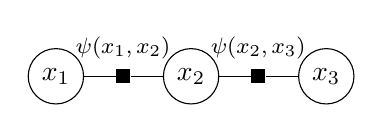
\begin{tikzpicture}
\node[latent] (x1) {$x_1$};
\node[latent, right=of x1] (x2) {$x_2$};
\node[latent, right=of x2] (x3) {$x_3$};
\factor[right=of x1] {f1} {$\psi(x_1,x_2)$} {} {};
\factor[right=of x2] {f2} {$\psi(x_2,x_3)$} {} {};
\factoredge {x1,x2} {f1} {};
\factoredge {x2,x3} {f2} {};
\end{tikzpicture}
\caption{
\label{fig:linear-chain}
}
\end{figure}

We compute the partition function as follows:
\begin{equation}
\begin{aligned}
Z
&= \sum_{x_1}\sum_{x_2} \psi_1(x_1, x_2) \sum_{x_3} \psi_2(x_2, x_3) \\
&\approx \sum_{x_1}\sum_{x_2} \phi(\bx_1)^T\phi(\bx_2) \sum_{x_3} \phi(\bx_2)^T\phi(\bx_3)\\
&= \left(\sum_{x_1} \phi(\bx_1)^T\right) \left(\sum_{\bx_2} \phi(\bx_2)\phi(\bx_2)^T\right)
    \left(\sum_{x_3}\phi(\bx_3)\right).
\end{aligned}
\end{equation}
We can precompute the sum of outer products $\sum_{\bx_2}\phi(\bx_2)\phi(\bx^T)$ independently,
resulting in time complexity $O(Td^2 + T|\mcX|d^2)$ in serial,
and $O(Td^2 + |\mcX|d^2)$ if the sums of outer products can be computed in parallel.
We can also apply a divide-and-conquer approach to further
reduce time to $O(c_{\textrm{mm}}(\log T + \log |\mcX|))$ on a parallel machine,
where $c_{\textrm{mm}}$ is the cost of a matrix multiplication.

\paragraph{Matrix version}
Probably much clearer here too.
todo

\subsection{Approximation error}
todo

\section{Application to PCFGs}
todo

\subsection{Approximation error}
todo

\bibliographystyle{plainnat}
\bibliography{bib}

\end{document}
